\subsection{SSC Mourning Cloak}

\begin{center}
    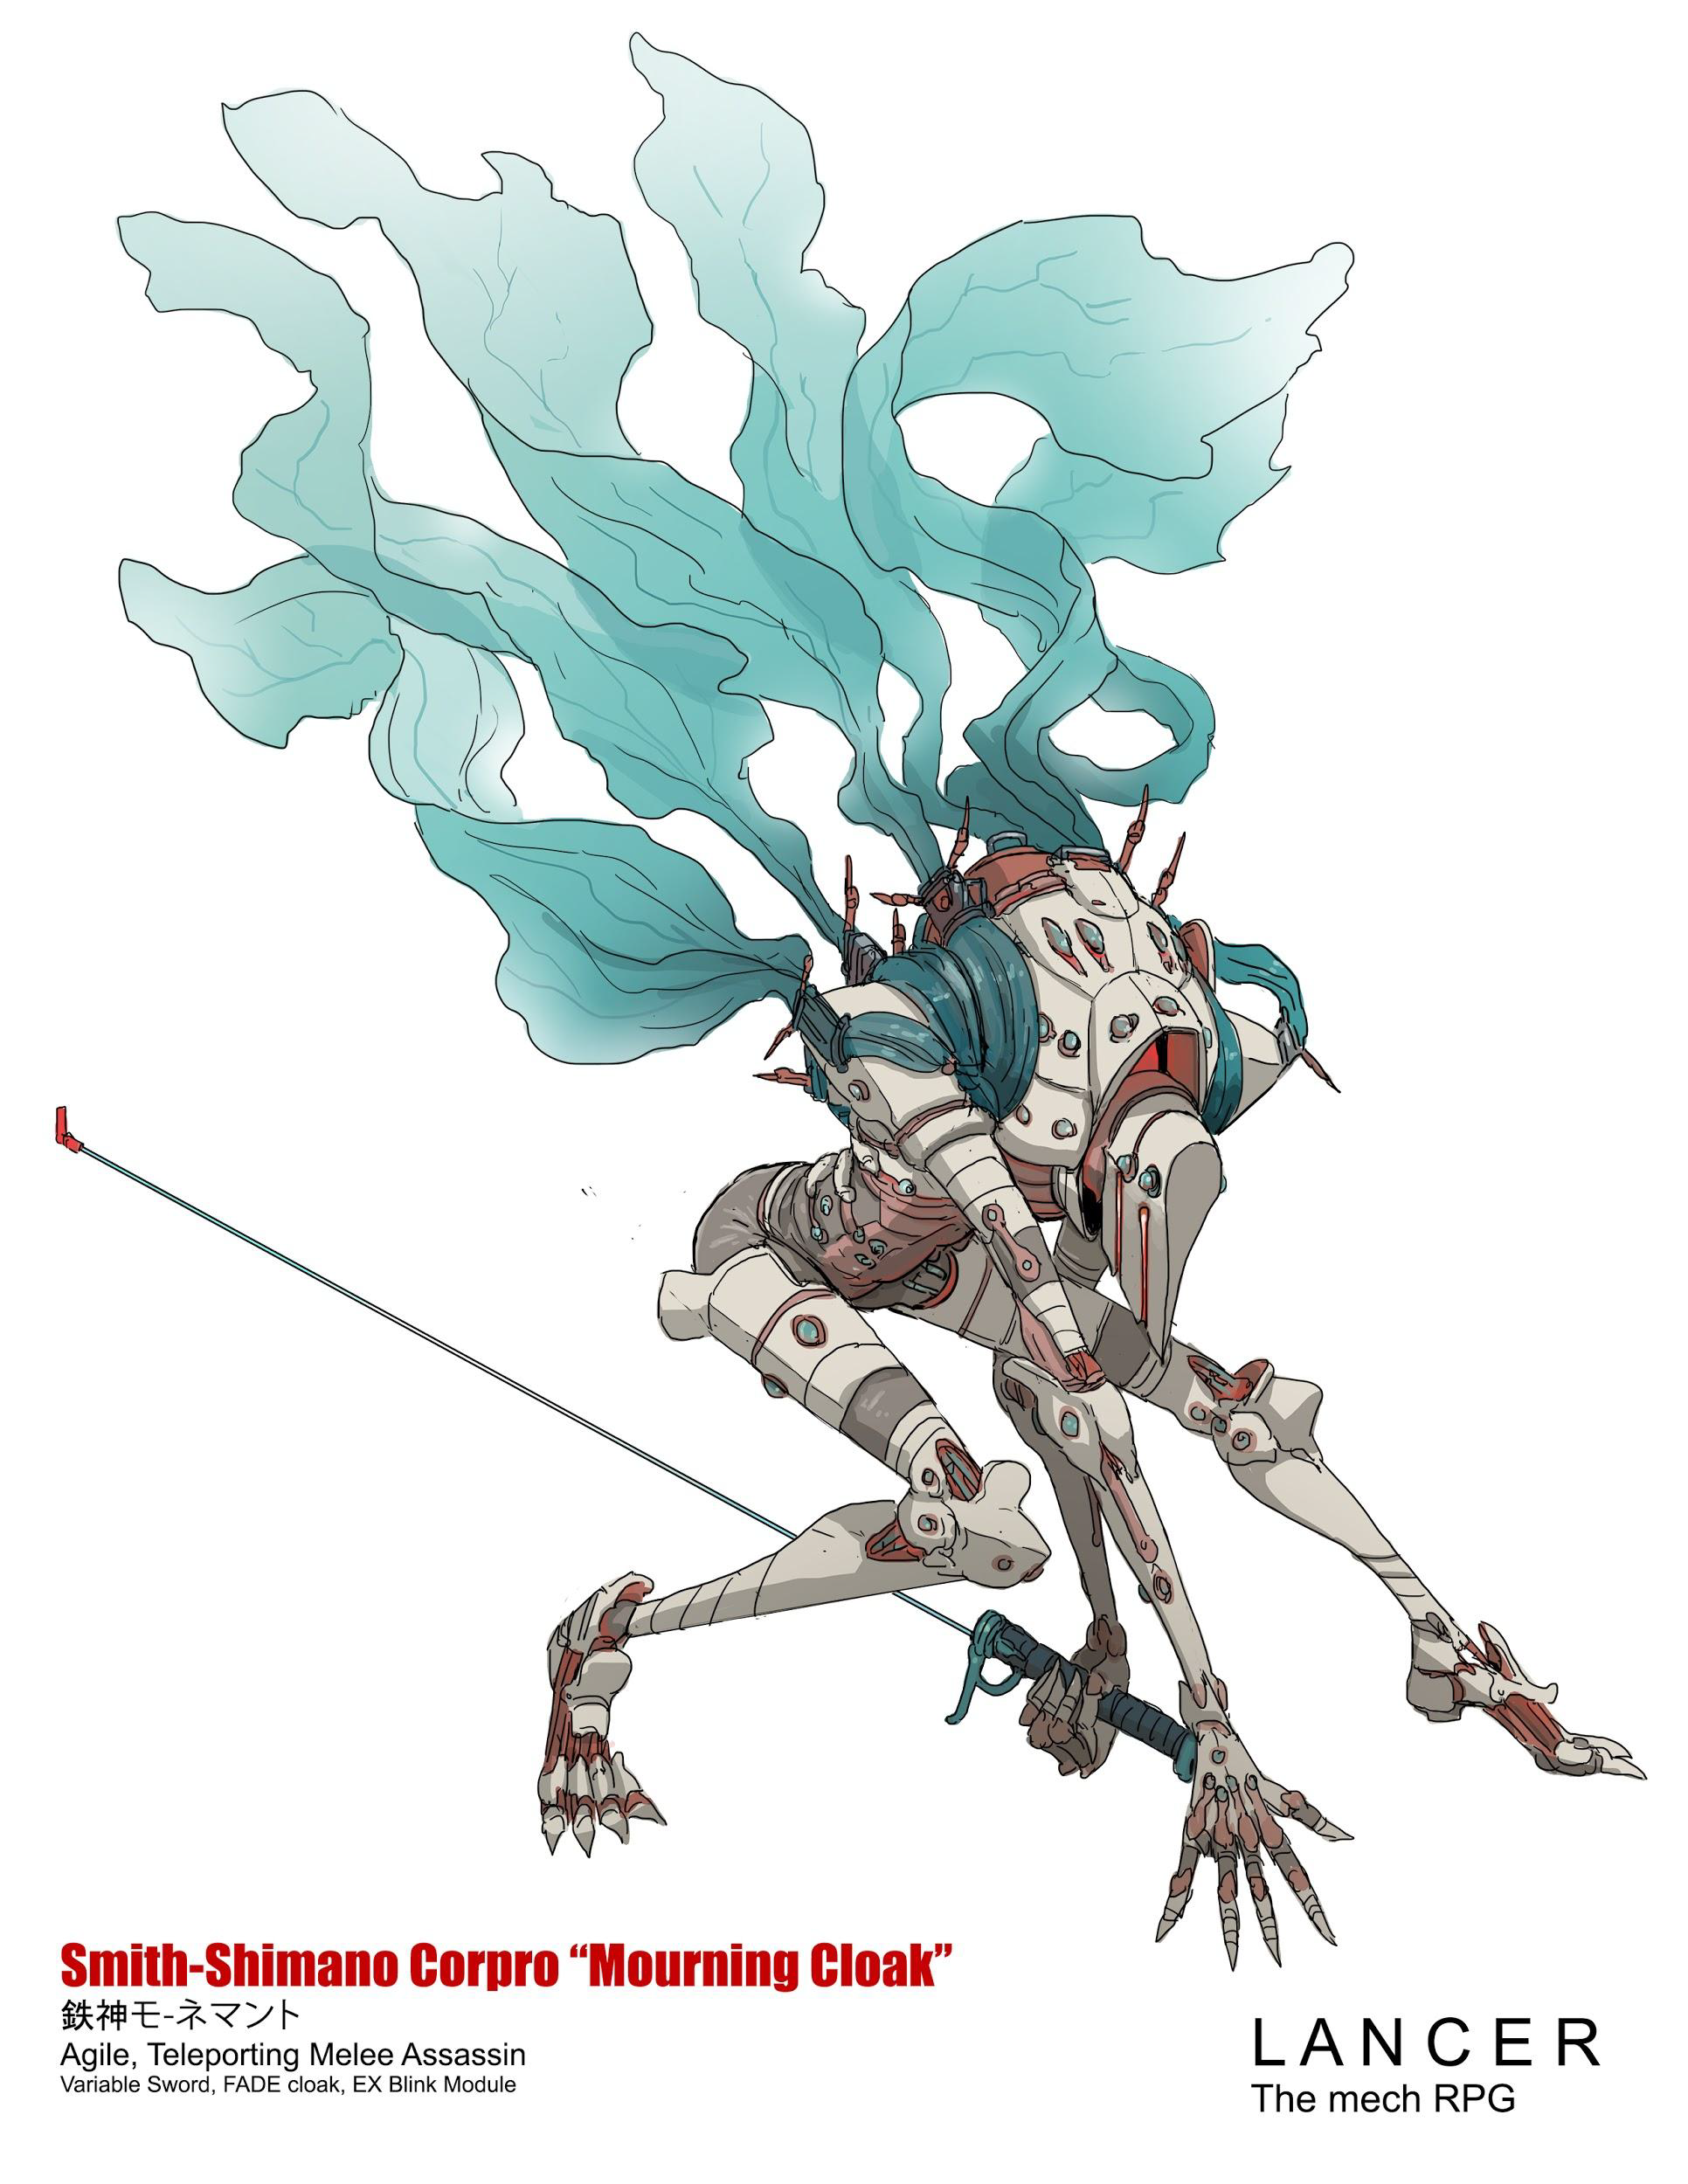
\includegraphics{MourningCloak}
\end{center}

\begin{mech}{SSC}{Mourning Cloak}

\fluff{The SSC MOURNING CLOAK core is intended to provide pilots with a closer-than-CQB tactical option for situations where firearms and ordnance weapons are impractical or unavailable. The MOURNING CLOAK line specializes in precision melee combat and is commonly outfitted with a complement of variable weaponry; shielded microfilament wires designed to attack vulnerable joints and external modules.}

\begin{license}
\item Variable Knife, Vijaya Rockets
\item Mourning Cloak FRAME, Exposed Singularity, Hunter Logic
\item Variable Sword, FADE Cloak
\end{license}
\frameBox
[hp = 8,
evasion = 12,
speed = 5,
heat cap = 4,
sensors = 10,
armor = 0,
e-defense = 6,
size = 1,
repair cap = 3,
tech attack = +1,
traits = {\textbf{Hunter:} The Mourning Cloak’s melee attacks become AP and deal +1d6 bonus damage if it is the only actor (allied or enemy) in engagement with the target

\textbf{Bioplating:} The Mourning Cloak gets +1 accuracy on agility checks},
sp = 6,
mount one = main/aux mount,
mount two = flex mount,
core system name = Smith-Shimano EX Slipstream Module,
core system text = {The EX SLIPSTREAM program is a Smith-Shimano innovation open only to highly licensed pilots. An interesting development in personal travel, the EX SLIPSTREAM module itself is a miniaturized near- lightspeed star drive capable of transporting the user through blinkspace with acceptable accuracy. The program and its technology is temperamental; a mech core is the smallest unit capable of surviving the stress of exposed blink travel, though the experience is still traumatic to the user and those in close proximity to egress.
Passive:
This dangerous and experimental module is a miniaturized starship nearlight drive. You can use it instead of moving or taking the boost action. When you use it, roll 3d6. You can teleport to a point within that range around you as long as there is space for your mech. You don’t have to be able to see this point, but if you attempt to teleport to an already occupied space (by terrain, another mech, etc), the teleport fails and you take 2d6 kinetic damage.
If you roll triples for this system, your mech disappears and does not re-appear, either indefinitely or until your party rests (up to you).},
core active name = Stabilize singularity,
core active text = {Active: Requires 1 core power
Protocol
Until the end of this scene, when you move or boost, you instead teleport up to the same distance.}]


Vijaya Rockets

Vijaya rockets are miniaturized, close range missiles fired from a portable, drum-fed launcher. Their shaped charges are formed in such a way as to project their blast forward, away from the user, and are intended for use in close range engagements as a force multiplier.

Auxiliary Launcher

Range 5

Accurate

1d3 explosive damage


Variable Knife

A variable knife is a shorter version of a variable sword, a shielded length of mono-molecular wire. The power drain on a mech’s systems makes mounting these weapons incredible taxing.

Auxiliary Melee

Accurate

Threat 1

2 kinetic damage

The Variable knife deals +1d3 bonus damage on critical hits

Exposed Singularity

SSC’s Exotic Materials project worked to develop the Mourning Cloak’s unique gravatic power plant. For the second generation of the SSC-MC, the Exotic Materials project devised a system that allows pilots to aperture open, for a moment, the gravatic containment system, exposing a slice of naked singularity to realspace. Naked singularity is difficult for organics and synthetics to perceive, being similar to the core of a black hole. The sudden exposure directed at foes (or other targets) essentially ``blanks'' the Mourning Cloak from real time. The Cloak’s pilot, meanwhile, experiences roughly 10 seconds of normal subjective time, allowing them a brief window in which they can act independently of local realtime. SSC does not recommend abusing this system, as the Exotic Materials group is still testing long-term exposure to local sidereal time.

2 SP, Unique

Reaction

Once per round, when your mech takes damage, you can immediately teleport up to 1d6 spaces as a reaction in a direction of your choosing (though if this teleport would put you inside an obstacle or other mech you take damage as normal and the teleport fails).


Hunter Logic
Building from interpreted strands of DHIYED-strain viral code, SSC’s Hunter Logic is an agile computational memetic, a dual synthetic/VLS-vector systemic weapon capable of crippling a target’s computer and crew.

2 SP


Quick Tech
Gain the following options for invasion:
         - Stalk Prey: Your systems infect the target with a viral logic that wipes your image from their sensors. Until you are damaged by that target, they count you as invisible. This system can only affect one target at a time (other targets still count you as visible and can see you normally).

	        - Terrify: Your systems infect the target with a viral logic that causes your mech to appear horrifying to the target. Until the end of its next turn, your target is impaired and also cannot willingly make any movement that would take it closer to you.


Variable Sword

The variable sword is a Smith-Shimano hallmark. A length of razor sharp molecular wire attached to a handle and caught in a magnetic field, a variable sword is invisible to the naked eye until it makes cuts in an enemy. Built in the early days of interstellar travel, the variable sword was meant to allow for precision sample gathering in the field, while also reducing the overall payload on a mech core.

Main melee

Accurate

Threat 2

3 kinetic damage.

The Variable Sword deals +1d6 bonus kinetic damage on critical hits


FADE Cloak




Representing SSC’s first successful manipulation of what the Aun call the ``Firmament'', each Firmament Affinity/Directed Entropy Drive must be fabricated to the unique firmament signatures of the pilot cleared to requisition it. FADE drives are rough tools, artificial affinity generators that allow operators to ``shimmer'', to nudge their physical bodies between the causal and paracausal. The drive extrudes a semi-organic membrane that accomplishes this effect, wrapping around the mech. At present, the long-term effects of this system on organic matter is unknown; pilots who are cleared to operate this system agree to check in with their SSC personal concierge on a regular schedule (``check in'' includes regular deposits of genetic material).

2 SP
Quick Action, Unique
Once this highly experimental drive is activated as an action, it shifts its user partially in and out of blinkspace. When activated, you immediately go out of phase with reality. While out of phase, you can ignore obstructions such as walls or cover and pass through enemy mechs and solid obstacles as if they were not there, but not end your turn there. You cannot interact with the physical world, but neither can it affect you (in terms of damage, etc). If for any reason you are forced to return while inside of another object, take 2d6 AP kinetic damage and return in the nearest available space.


At the start of each of your turns while this system is active, roll a d6. On a 4+, you go or remain out of phase, on a 3 or lower, you return to the battlefield until the start of your next turn. This drive can’t be activated again if it’s already active. It deactivates if you make an overheating check, deactivate as a quick action, or the scene ends.
\end{mech}